\section{Scene backgrounds}
\label{app:Scenes}

The images used as a test for background noise when detecting images.


\section{Robotics Plots}
\label{app:roboticsPlots}

\subsection{Robot Configurations}
Robot configurations of the robot when tracking one or three points at the three different speeds.
\begin{figure}[H]
\centering
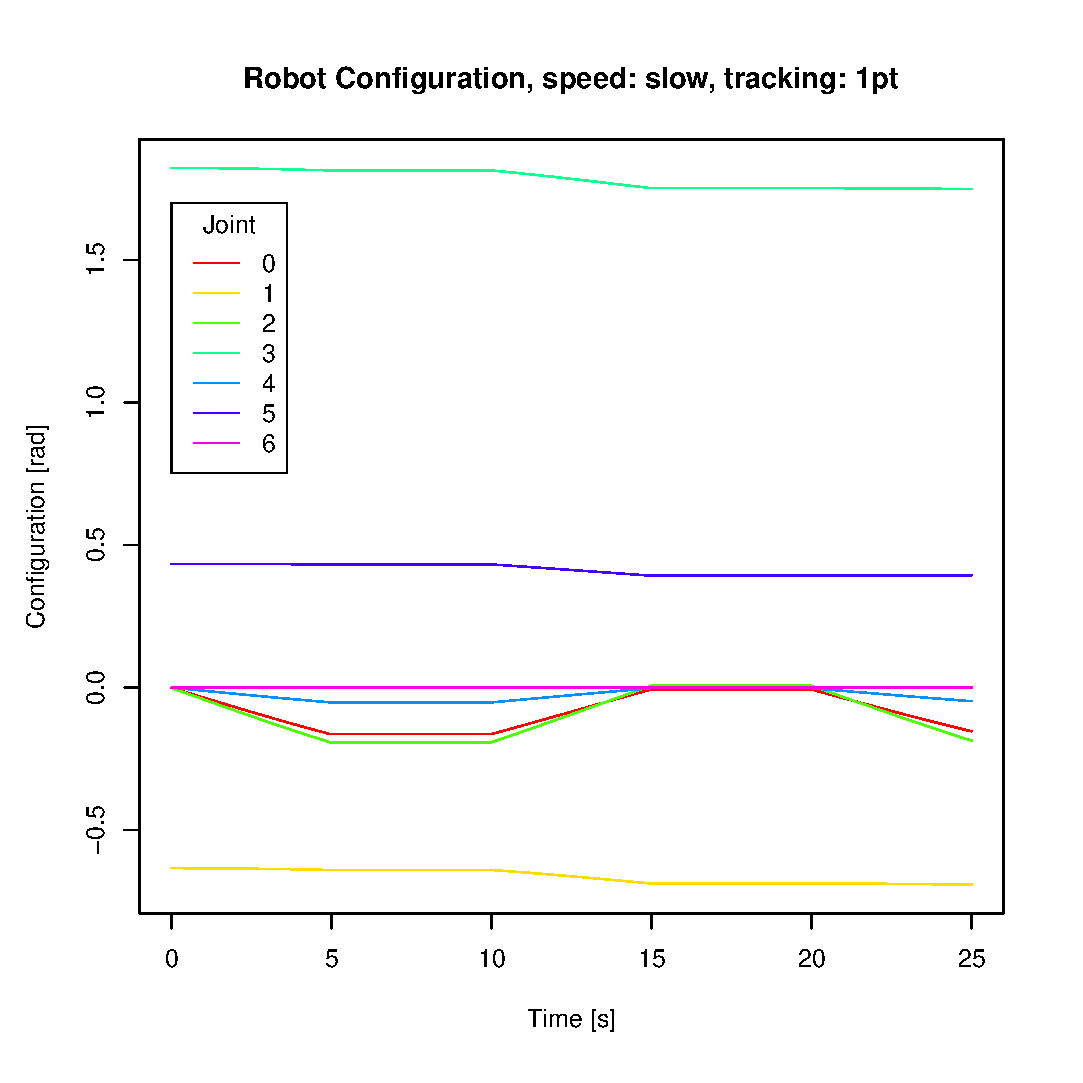
\includegraphics[width= \linewidth]{graphics/robotics/robotConfiguration_slow_1pt}
\caption{}
\label{fig:}
\end{figure}

\begin{figure}[H]
\centering
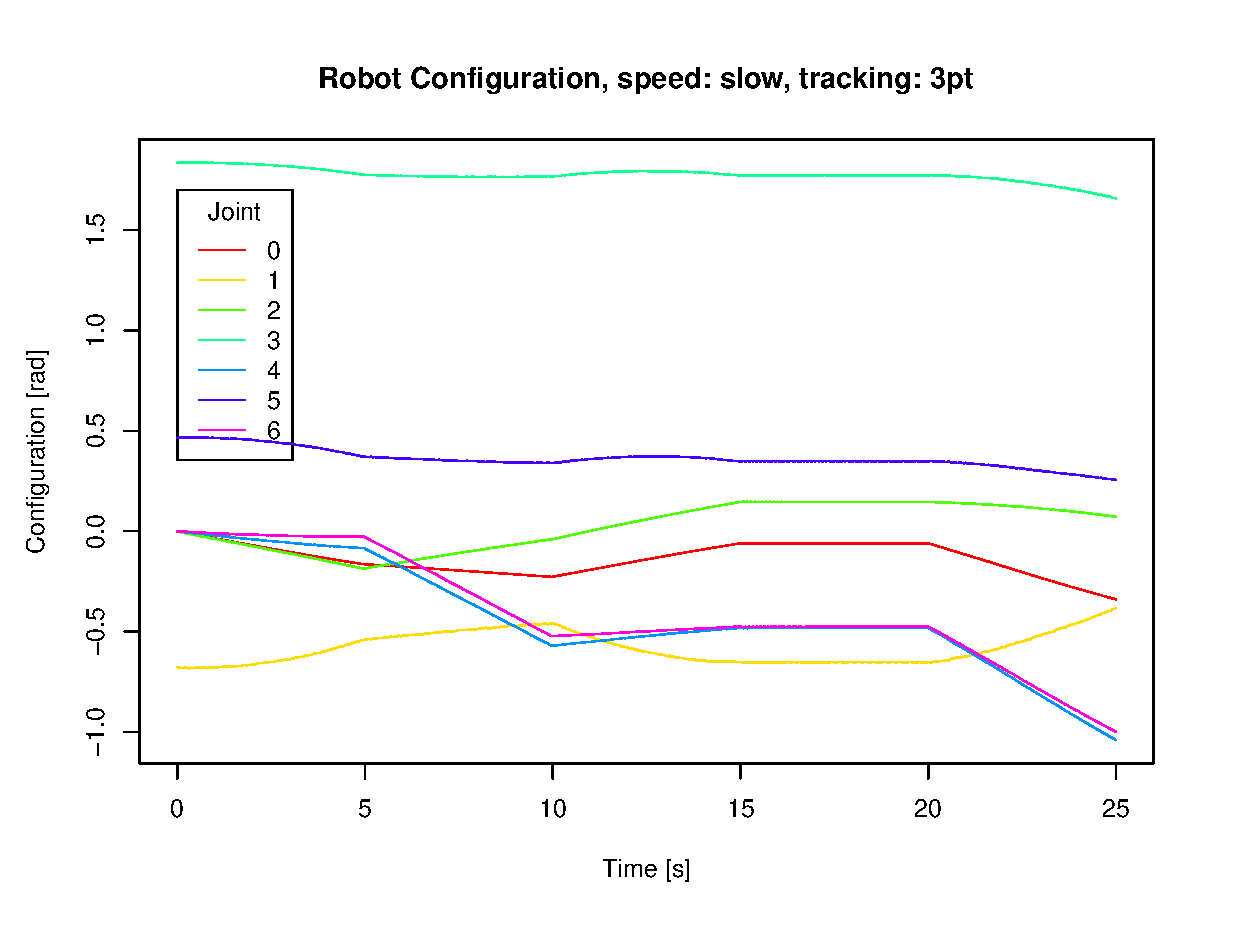
\includegraphics[width= \linewidth]{graphics/robotics/robotConfiguration_slow_3pt}
\caption{}
\label{fig:}
\end{figure}

\begin{figure}[H]
\centering
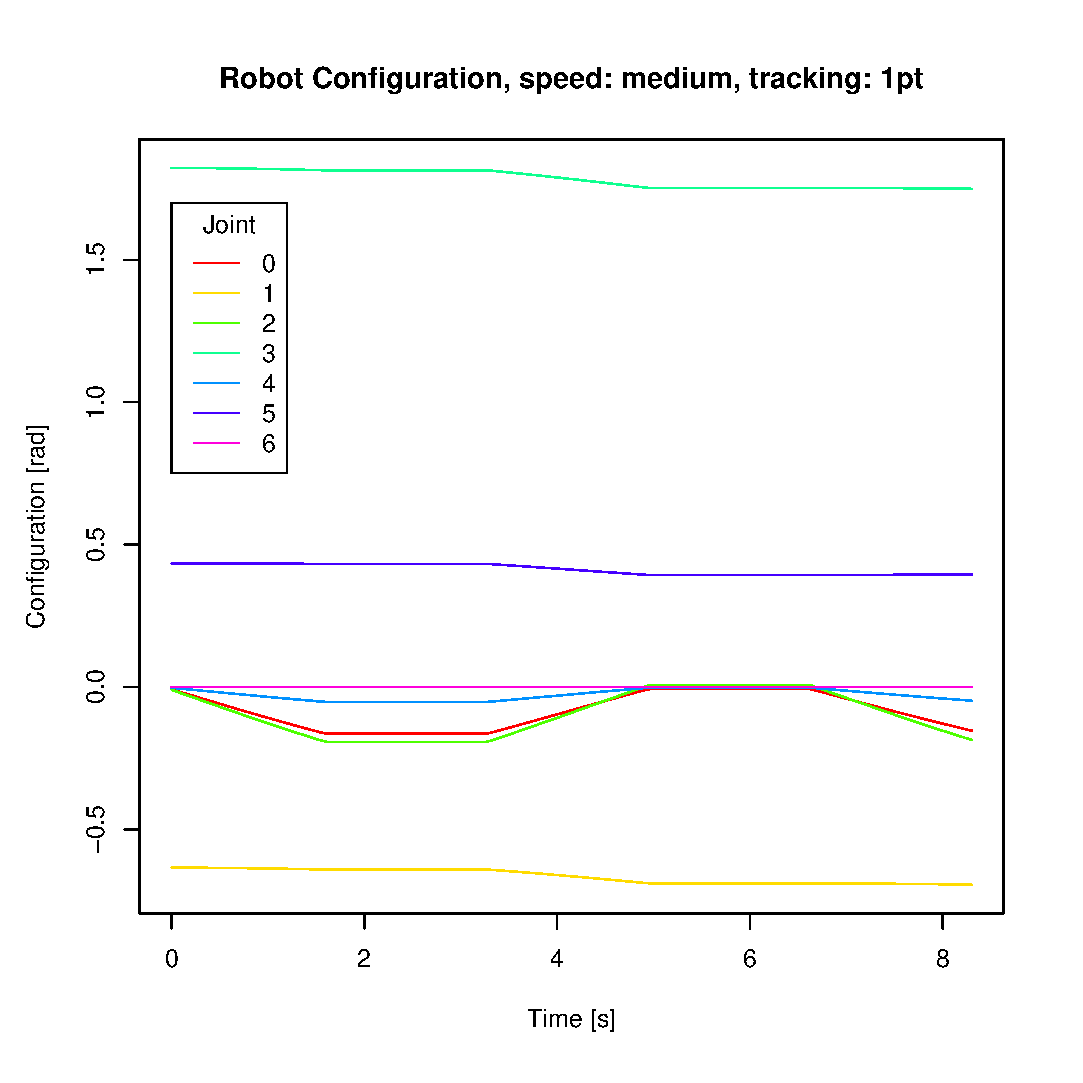
\includegraphics[width= \linewidth]{graphics/robotics/robotConfiguration_medium_1pt}
\caption{}
\label{fig:}
\end{figure}

\begin{figure}[H]
\centering
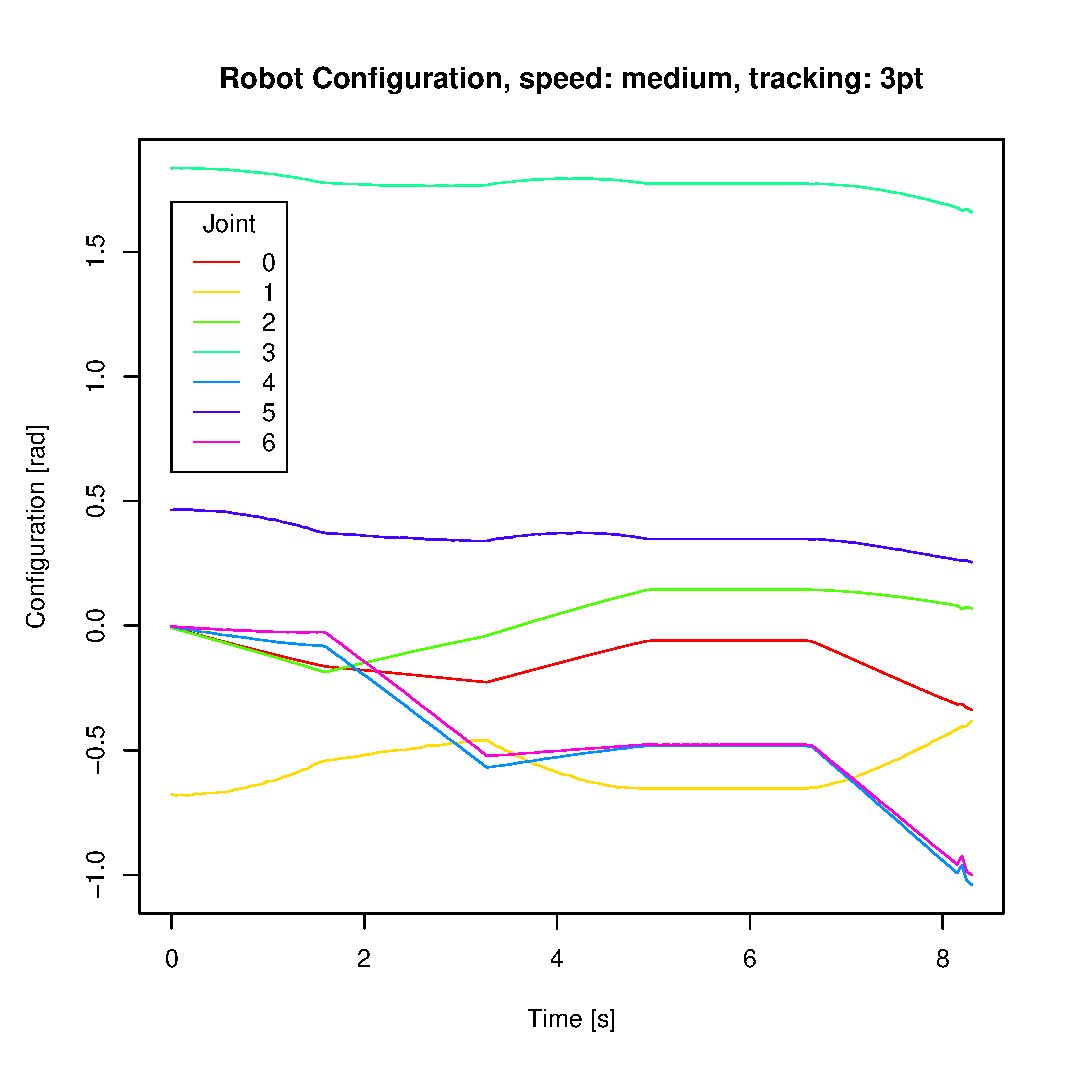
\includegraphics[width= \linewidth]{graphics/robotics/robotConfiguration_medium_3pt}
\caption{}
\label{fig:}
\end{figure}

\begin{figure}[H]
\centering
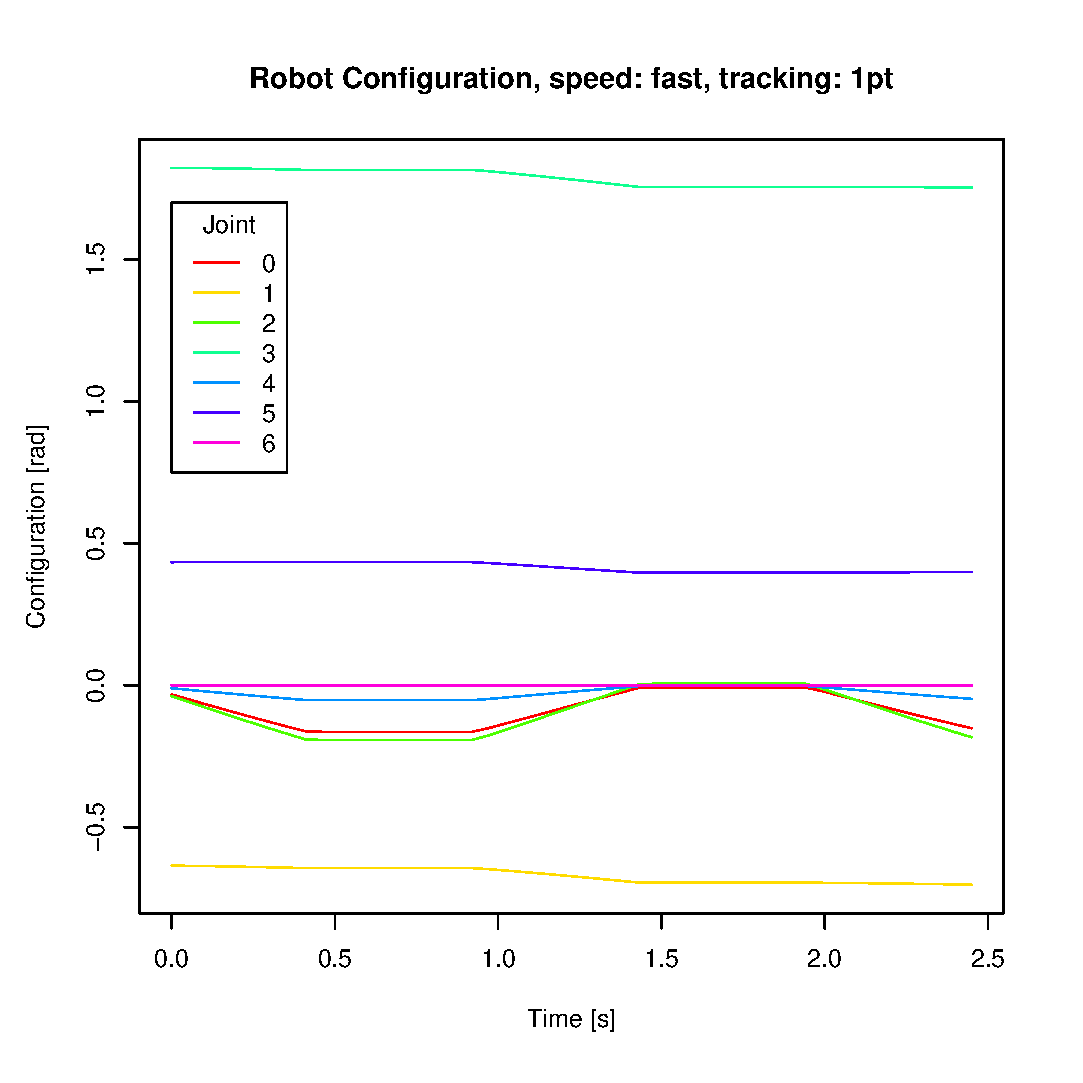
\includegraphics[width= \linewidth]{graphics/robotics/robotConfiguration_fast_1pt}
\caption{}
\label{fig:}
\end{figure}

\begin{figure}[H]
\centering
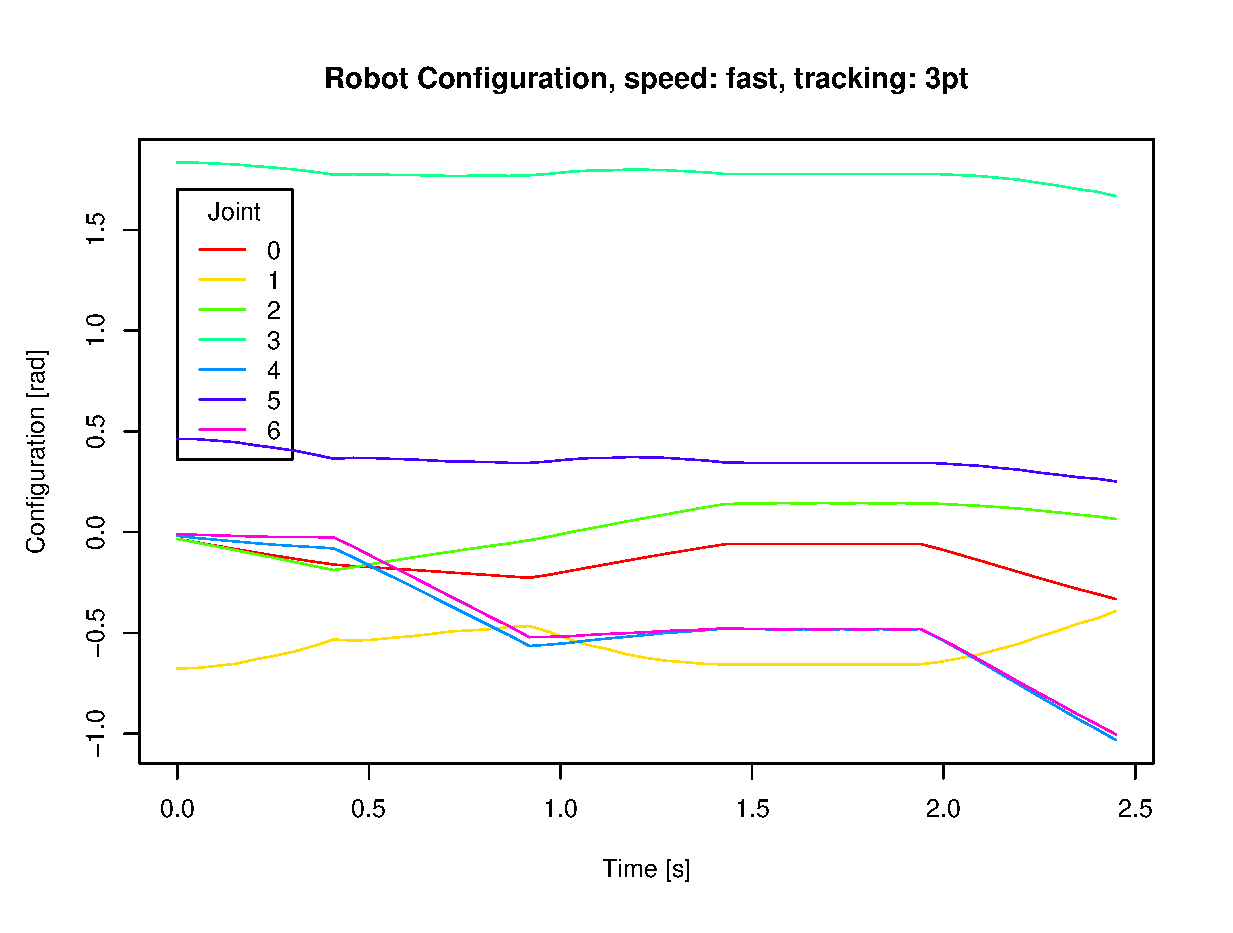
\includegraphics[width= \linewidth]{graphics/robotics/robotConfiguration_fast_3pt}
\caption{}
\label{fig:}
\end{figure}


